\documentclass{article}
\usepackage[final]{neurips} % ready for submission, but you have multiple options to import this
\usepackage[utf8]{inputenc} % allow utf-8 input
\usepackage[T1]{fontenc}    % use 8-bit T1 fonts
\usepackage{hyperref}       % hyperlinks
\usepackage{url}            % simple URL typesetting
\usepackage{booktabs}       % professional-quality tables
\usepackage{amsfonts}       % blackboard math symbols
\usepackage{nicefrac}       % compact symbols for 1/2, etc.
\usepackage{microtype}      % microtypography
\usepackage{xcolor}         % colors
\usepackage{graphicx}
\usepackage{subfigure}
\usepackage[backend=biber,style=numeric]{biblatex}
\addbibresource{references.bib} % Replace with your .bib file name

\begin{document}

\title{Soccer Sage: Forecasting the Future of Soccer}

\author{%
    GroupID: P28
    \AND
  Abhishek Rao \\
  \texttt{arao23@ncsu.edu} \\
  \And
  Manav Divyesh Shah \\
  \texttt{mdshah5@ncsu.edu} \\
  \And
  Srimadh Vasuki Rao \\
  \texttt{svrao3@ncsu.edu}
}


\maketitle

%%%%%%%%%%%%%%%%%%%%%%%%%%%%%%%%%%%%%%%%%%%%%%%%%%%%%%%%%%%%%%%%%
%%%%%%%%%%%%%%%%%%%%% --- SECTION START --- %%%%%%%%%%%%%%%%%%%%%
%%%%%%%%%%%%%%%%%%%%%%%%%%%%%%%%%%%%%%%%%%%%%%%%%%%%%%%%%%%%%%%%%
\section{Background and Introduction}
\label{gen_inst}

Data analysis has become a cornerstone of decision-making in modern sports, particularly in soccer. The immense volume of data generated in the sport—including over 3 million data points per match, more than 75 metrics per player, and a transfer market valued at over 10 billion euros—provides an opportunity to derive actionable insights. Soccer clubs increasingly rely on data to improve performance, predict match outcomes, and optimize player transfers. A prime example is Liverpool FC, which employed a data-driven approach to identify undervalued talent, address team weaknesses, and build a title-winning squad.

The general problem our project addresses is the use of data analysis and machine learning to enhance decision-making in soccer. Specifically, we aim to achieve two key objectives:
\begin{enumerate}
    \item Predicting the \textbf{outcomes of soccer matches.}
    \item Identifying \textbf{suitable player transfers} to strengthen teams by addressing their weaknesses.
\end{enumerate}

In this project, we have explored innovative ways to combine historical match outcomes, player statistics, and team dynamics to enhance prediction accuracy and player evaluation. It aims to not only replicate but improve upon existing methodologies by incorporating modern machine learning approaches and comprehensive exploratory data analysis (EDA). These efforts yield insights that are both academically valuable and practically applicable for soccer teams.

Prior work on predicting soccer match outcomes and player performance offers a range of methodologies and varying degrees of success:

Hervert-Escobar et al. \cite{hervert2018} proposed a bayesian learning model for match outcome prediction, achieving an accuracy of 47.92\%. Their work underscored the inherent uncertainty and stochastic nature of soccer games. Holmes and McHale \cite{holmes2024} introduced a player rating-based skellam model to forecast football match results. With an accuracy of 53.88\%, this approach demonstrated that individual player contributions can significantly impact prediction reliability. Ulmer et al. \cite{ulmer2013} developed multiple models, including Gaussian Naive Bayes, Hidden Markov Models, Linear SVM, and Random Forest, for predicting English Premier League match results with a modest accuracy of 50\%. This study highlighted the challenges of incorporating multiple complex factors into a prediction framework. 


The existing literature indicates a strong foundation for using data analysis in soccer, but challenges remain in improving prediction accuracy and translating insights into actionable strategies for player transfers. Our project builds upon these efforts by leveraging the European Soccer Database (2008--2016), a comprehensive resource encompassing match outcomes, player statistics, and team data from multiple European leagues. By applying exploratory data analysis (EDA) and machine learning techniques, we aim to improve prediction models and develop an efficient framework for identifying suitable player transfers.

%%%%%%%%%%%%%%%%%%%%%%%%%%%%%%%%%%%%%%%%%%%%%%%%%%%%%%%%%%%%%%%%%
%%%%%%%%%%%%%%%%%%%%% --- SECTION START --- %%%%%%%%%%%%%%%%%%%%%
%%%%%%%%%%%%%%%%%%%%%%%%%%%%%%%%%%%%%%%%%%%%%%%%%%%%%%%%%%%%%%%%%
\section{Methods}

\subsection{Random Forest Classifier}
\begin{itemize}
    \item \textbf{Approach:} Random Forest is an ensemble learning method that constructs multiple decision trees during training and aggregates their predictions (majority vote for classification) to improve generalization and reduce overfitting. Each tree is trained on a bootstrap sample with a random subset of features.
    \item \textbf{Parameters:} \texttt{n\_estimators=500}, \texttt{class\_weight='balanced'}.
    \item \textbf{Rationale}: Random Forest was chosen over decision trees due to its ability to reduce overfitting by averaging multiple trees, which improves generalization. Additionally, its implicit feature selection reduces the need for extensive preprocessing, making it computationally efficient. Decision trees alone tend to overfit the training data, which is why Random Forest serves as a better alternative.
\end{itemize}

\subsection{Gradient Boosting Classifier}
\begin{itemize}
    \item \textbf{Approach:} Gradient Boosting is an iterative approach that trains weak learners sequentially, each correcting the errors of the previous model by optimizing a loss function. This method uses decision trees as base learners and focuses on reducing residual errors.
    \item \textbf{Parameters:} \texttt{n\_estimators=500}.
    \item \textbf{Rationale}: Gradient Boosting was included for its ability to achieve high accuracy, especially for complex data patterns. By sequentially correcting residual errors, it complements Random Forest and strengthens the ensemble's predictive performance. Unlike Random Forest, which works in parallel, Gradient Boosting’s sequential nature provides a more fine-tuned approach.
\end{itemize}

\subsection{Neural Network with CrossEntropy Loss}
\begin{itemize}
    \item \textbf{Approach:} A simple feedforward neural network with two hidden layers containing of 64 and 32 neurons was implemented. The model was trained using backpropagation with a CrossEntropy loss function to minimize classification error.
    \item \textbf{Parameters:} \texttt{hidden\_layer\_sizes=(64, 32)}, \texttt{max\_iter=50}.
    \item \textbf{Rationale}: Neural Networks were included to handle non-linear relationships and learn complex data representations. During experimentation, larger architectures were tried, but they suffered from significant overfitting, particularly failing to predict the "Draw" class. This motivated the choice of smaller architectures. A simple architecture with CrossEntropy Loss was used as a baseline to limit computational overhead. We also implemented a PyTorch-based model with Focal Loss specifically addressed class imbalance, focusing on hard-to-classify samples. Dropout layers improved generalization, and the architecture was designed to balance computational complexity with performance. But this approach led to a reduction in the final accuracy and was computationally expensive due to which we did not include this approach in the final approach. 
\end{itemize}

\subsection{Ensemble Model with Soft Voting}
\begin{itemize}
    \item \textbf{Approach:} An ensemble method combining Random Forest, Gradient Boosting, Gaussian Naive Bayes, and Support Vector Machine (SVM) using soft voting. The method aggregates probabilities from all models and selects the class with the highest aggregated probability.
    \item \textbf{Parameters:} 
    \begin{itemize}
        \item \texttt{Random Forest: n\_estimators=500, class\_weight='balanced'}.
        \item \texttt{Gradient Boosting: n\_estimators=500}.
        \item \texttt{SVM: kernel='rbf', C=0.5, gamma=0.1}.
    \end{itemize}
    \item \textbf{Rationale}: The ensemble method combines the strengths of multiple classifiers. Random Forest and Gradient Boosting provide robustness to overfitting and high accuracy. SVM contributes a non-linear perspective with its kernel trick, and Gaussian Naive Bayes adds simplicity and efficiency for linearly separable classes. Soft voting was chosen over hard voting to leverage probabilistic predictions, improving the model's ability to balance between all classes.
\end{itemize}

Approaches like k-Nearest Neighbors (k-NN) and single decision trees were not pursued due to their computational inefficiency with large datasets and tendency to overfit. Support Vector Machines were only included within the ensemble due to their computational cost when used individually for multiclass problems. Logistic Regression was also considered but was deemed less suitable for capturing complex non-linear relationships.

%%%%%%%%%%%%%%%%%%%%%%%%%%%%%%%%%%%%%%%%%%%%%%%%%%%%%%%%%%%%%%%%%
%%%%%%%%%%%%%%%%%%%%% --- SECTION START --- %%%%%%%%%%%%%%%%%%%%%
%%%%%%%%%%%%%%%%%%%%%%%%%%%%%%%%%%%%%%%%%%%%%%%%%%%%%%%%%%%%%%%%%
\section{Plan and Experiment}

\subsection{Hypotheses}

The primary questions investigated in this project are:
\begin{enumerate}
    \item Can we predict match outcomes using the features in the dataset? 
    \item Can we identify optimal player transfers to strengthen a team based on player statistics and team needs?
\end{enumerate}

These hypotheses explore the potential of the European Soccer Dataset for predictive and prescriptive analytics. The insights gained from exploratory data analysis (EDA) provide valuable guidance for addressing these questions.

\subsection{Datasets}

The project utilizes the European Soccer Database, which includes detailed match data, player attributes, and team statistics from the top 5 European leagues: English Premier League, Spanish La Liga, German Bundesliga, Italian Serie A, and French Ligue 1. The dataset is structured into interconnected tables, including:
\begin{itemize}
    \item \textbf{Matches:} Comprehensive details of matches, including date, venue, teams, scores, and match statistics like possession percentage and shots.
    \item \textbf{Teams:} Club-level attributes, including styles of play in attack and defense.
    \item \textbf{Players:} Player profiles with personal details, physical attributes, and performance metrics.
    \item \textbf{Player Attributes:} Skills like passing accuracy, shooting ability, defensive prowess, and overall rating.
\end{itemize}

The dataset provides a robust foundation for testing the hypotheses.

\subsubsection{Data Preprocessing and Transformation}

To ensure the quality and consistency of the data, several preprocessing steps were performed:
\begin{enumerate}
    \item \textbf{Handling Missing Values:} Missing values were imputed using the average fill method, ensuring consistent data quality.
    \item \textbf{Feature Aggregation:} Player and team-level data were aggregated to compute performance metrics over multiple seasons.
    \item \textbf{Feature Engineering:}
    \begin{itemize}
        \item \textbf{Team Performance Metrics:} Aggregated player ratings to derive home and away team ratings as continuous ratio attributes.
        \item \textbf{Match Outcome Encoding:} Encoded outcomes as categorical variables: Home Win (1), Draw (0), and Away Win (-1).
        \item \textbf{Tactical Attributes:} One-hot encoded categorical attributes like playing style and tactical approaches. Numerical features such as build-up play, chance creation, and defensive metrics were retained for predictive modeling.
    \end{itemize}
\end{enumerate}

\subsection{Experimental Design}

\subsubsection{Hypothesis 1: Predicting Match Outcomes}
The goal is to evaluate whether match outcomes can be accurately predicted using team and match-level features.
\begin{itemize}
    \item \textbf{Plan:} Train predictive models, including Random Forest, Gradient Boosting, and Neural Networks, using features derived from EDA and correlation analysis. Evaluate performance using metrics such as Accuracy, Precision, Recall, and F1-Score.
    \item \textbf{EDA Insights:} 
    \begin{itemize}
        \item Correlation analysis highlighted that team ratings and tactical metrics are strongly associated with match outcomes.
        \item League play style analysis showed that certain tactical metrics, such as passing and defensive attributes, vary by league and can influence match predictions.
    \end{itemize}
    \item \textbf{Challenges:} Class imbalance, particularly for the "Draw" class, may affect model performance. Overfitting was observed with larger neural networks, which failed to predict "Draws." Smaller architectures with class weighting were employed to mitigate this issue.
\end{itemize}

\subsubsection{Hypothesis 2: Identifying Optimal Player Transfers}
The aim is to classify players into roles (e.g., Creator, Finisher, Defender) and identify underperforming areas for a team to help fill in the gap.
\begin{itemize}
    \item \textbf{Plan:} Classify players based on player attributes using filtering techniques, and compare against team needs derived from performance gaps. Predict future player potential using linear regression analysis.
    \item \textbf{EDA Insights:}
    \begin{itemize}
        \item Figure~\ref{fig:players_skills} illustrates that metrics such as \textit{standing tackles}, \textit{sliding tackles}, and \textit{interceptions} showed bimodal distributions, distinguishing defensive players from others.General skills, such as \textit{shooting}, \textit{passing}, and \textit{agility}, followed a bell curve, highlighting their universal importance across player roles.
        \item League play style analysis revealed that La Liga teams emphasize passing for chance creation, while Bundesliga teams favor rapid buildup play. These insights can inform strategy development.
        \item Figure~\ref{fig:radar_plot} shows us that top-rated players tend to have balanced skill sets, suggesting that versatility is crucial.
    \end{itemize}
    \item \textbf{Challenges:} We saw that player roles are subjective and may not map directly to available features. We need expert analysis to identify which features map to what player roles. We also see that balancing historical performance with current form is critical for effective recommendations.
\end{itemize}


%%%%%%%%%%%%%%%%%%%%%%%%%%%%%%%%%%%%%%%%%%%%%%%%%%%%%%%%%%%%%%%%%
%%%%%%%%%%%%%%%%%%%%% --- SECTION START --- %%%%%%%%%%%%%%%%%%%%%
%%%%%%%%%%%%%%%%%%%%%%%%%%%%%%%%%%%%%%%%%%%%%%%%%%%%%%%%%%%%%%%%%
\section{Results}

\subsection{Match Outcome Prediction}

Table~\ref{tab:results_comparison} and Figure~\ref{fig:confusion_matrix} summarizes the performance of the models tested for match outcome prediction to address hypothesis 1. While the results indicate moderate success in predicting "Home Wins" and "Away Wins," they also highlight the significant challenge of predicting the "Draw" class due to its lower representation in the dataset. 

\begin{table}[htbp]
    \centering
    \caption{Comparison of Model Results}
    \resizebox{\textwidth}{!}{%
    \begin{tabular}{@{}lcccccccc@{}}
        \toprule
        \textbf{Metric} & \multicolumn{2}{c}{\textbf{Random Forest}} & \multicolumn{2}{c}{\textbf{Gradient Boosting}} & \multicolumn{2}{c}{\textbf{Neural Network}} & \multicolumn{2}{c}{\textbf{Ensemble}} \\
        \cmidrule(lr){2-3} \cmidrule(lr){4-5} \cmidrule(lr){6-7} \cmidrule(lr){8-9}
        & Accuracy & F1-Score & Accuracy & F1-Score & Accuracy & F1-Score & Accuracy & F1-Score \\
        \midrule
        Overall Accuracy & 0.4482 & 0.43 & 0.5043 & 0.42 & 0.5021 & 0.41 & 0.4929 & 0.43 \\
        \midrule
        \textbf{Class} & Precision & Recall & Precision & Recall & Precision & Recall & Precision & Recall \\
        \midrule
        Away Win & 0.41 & 0.38 & 0.49 & 0.35 & 0.46 & 0.37 & 0.46 & 0.38 \\
        Draw & 0.26 & 0.17 & 0.29 & 0.03 & 0.25 & 0.00 & 0.26 & 0.04 \\
        Home Win & 0.53 & 0.65 & 0.51 & 0.87 & 0.51 & 0.87 & 0.52 & 0.81 \\
        \midrule
        Macro Avg & 0.40 & 0.39 & 0.43 & 0.37 & 0.41 & 0.35 & 0.41 & 0.38 \\
        Weighted Avg & 0.42 & 0.43 & 0.45 & 0.42 & 0.43 & 0.41 & 0.43 & 0.43 \\
        \bottomrule
    \end{tabular}%
    }
    \label{tab:results_comparison}
\end{table}


The F1-score for the neural network is low compared to ensemble or Gradient boosting methods, showing us the importance of maintaining both good accuracy and good F-1 score.

The results mostly answered the question of whether match outcomes could be predicted using the dataset. While the models were effective at predicting “Home Wins” and “Away Wins,” the “Draw” class remained highly underrepresented, leading to poor recall and precision for this outcome. This indicates that while the models capture key patterns for certain match outcomes, the dataset’s imbalances and lack of dynamic, in-game contextual factors limit their overall performance.

The primary limitation lies in the dataset itself, the “Draw” class is underrepresented in the data, leading to biased predictions favoring more frequent outcomes.Also, the dataset lacks dynamic features such as in-game momentum, psychological factors, or real-time tactical adjustments, which play a crucial role in determining match outcomes.

To address the above issues, we can introduce new features like match importance, player fatigue, and home-crowd effects to capture contextual dynamics.We can also experiment with recurrent neural networks (RNNs) or transformers to model the sequential progression of a team performance in the year, to identify momentum and other factors within a match.

\begin{figure}
    \centering
    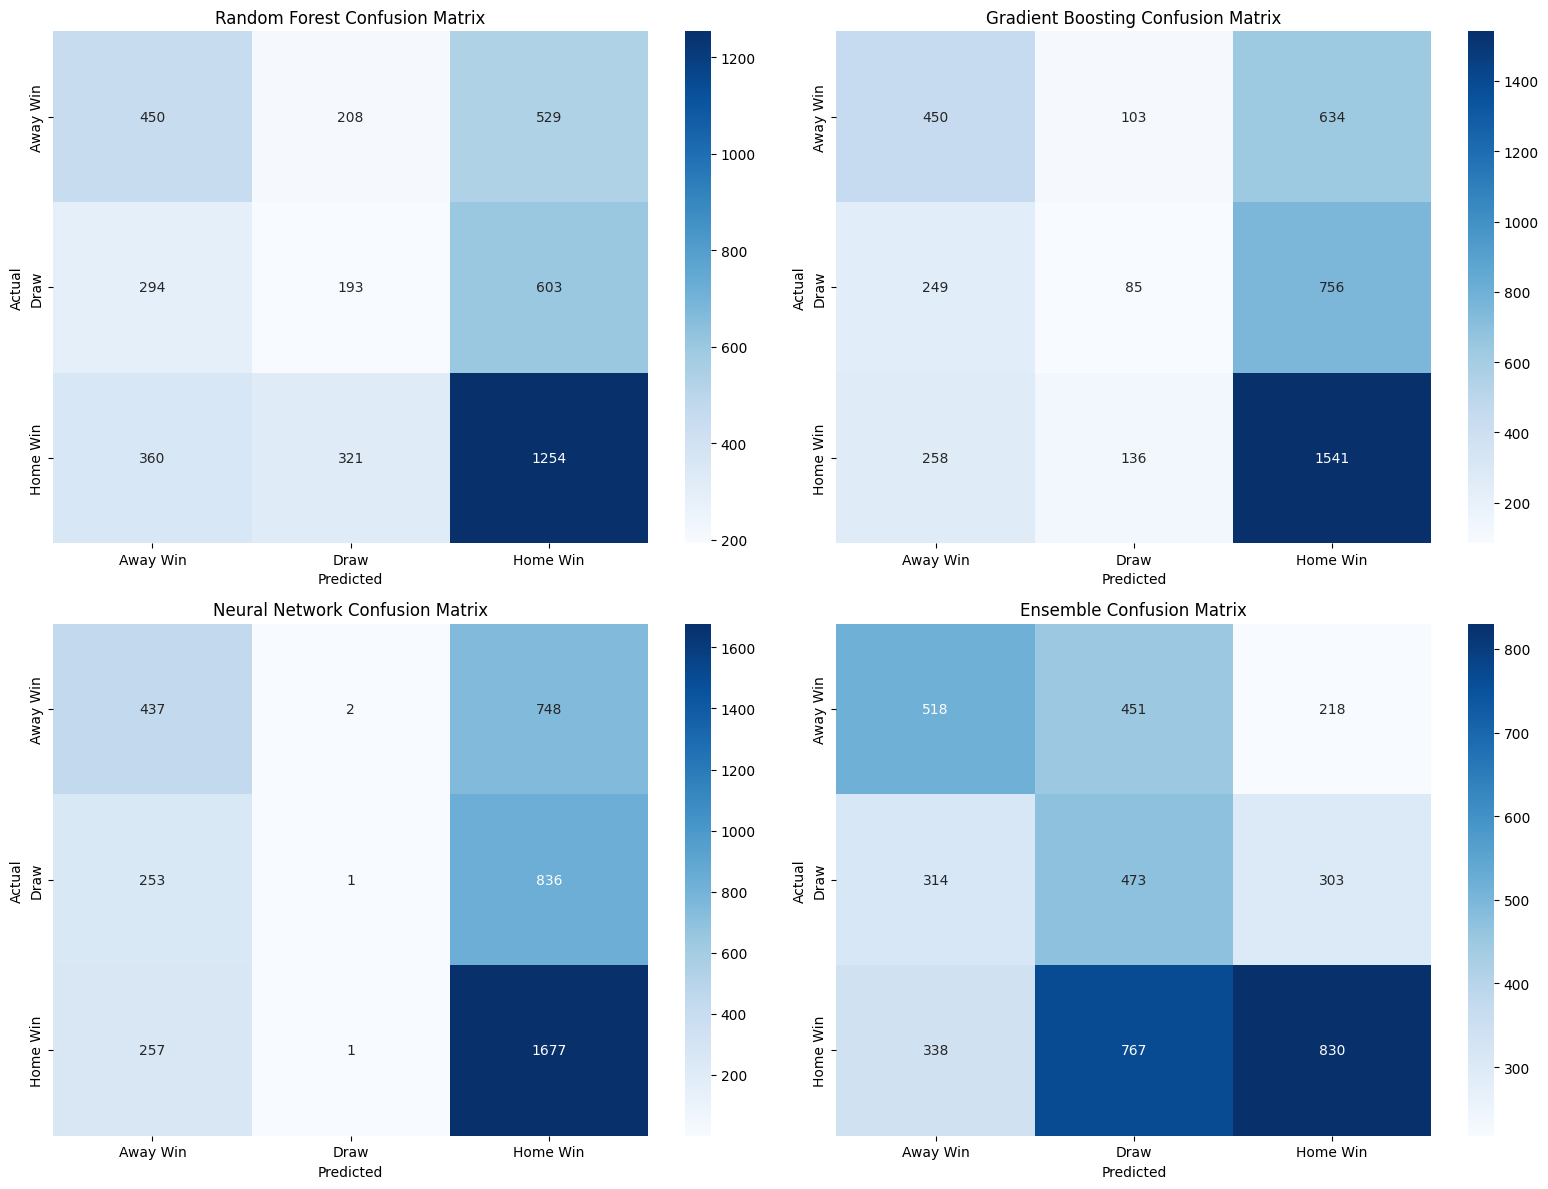
\includegraphics[width=1\linewidth]{confusion_matrix.png}
    \caption{Confusion matrix for match outcome predictions, illustrating model strengths in predicting wins and weaknesses in identifying draws}
    \label{fig:confusion_matrix}
\end{figure}
\begin{figure}
    \centering
    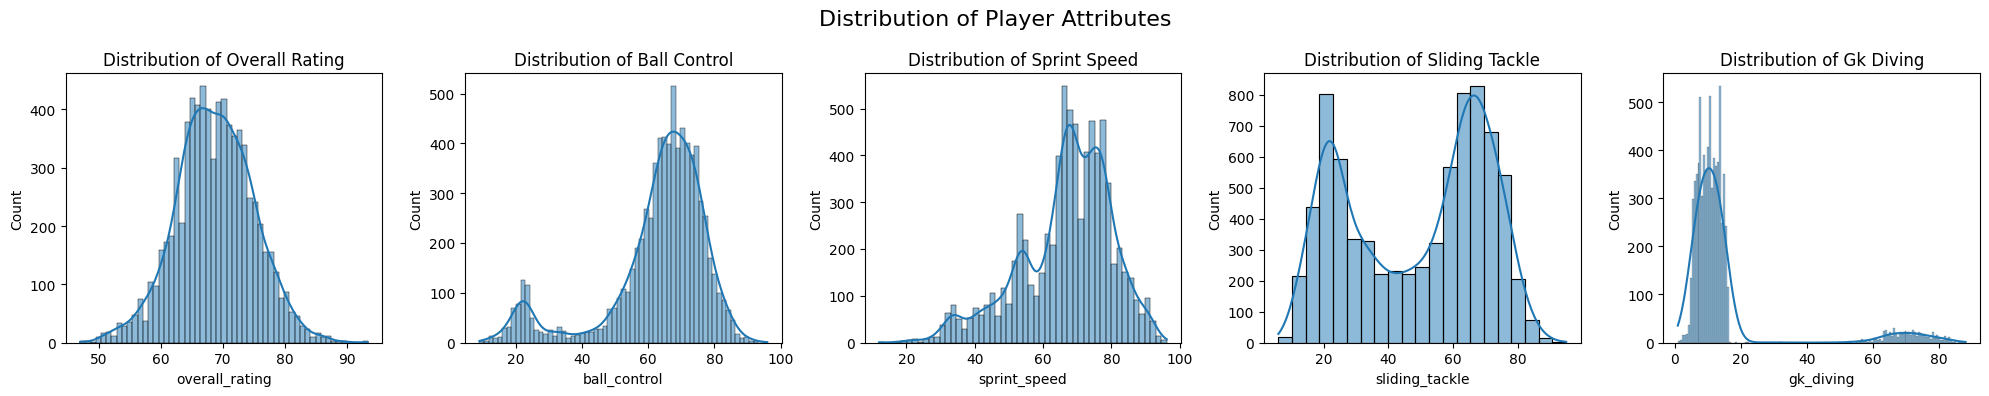
\includegraphics[width=1\linewidth]{players_skill.png}
\caption{Player skills show distinct patterns: bell-shaped for universal attributes, bimodal for defensive metrics}
    \label{fig:players_skills}
\end{figure}

\begin{figure}
    \centering
    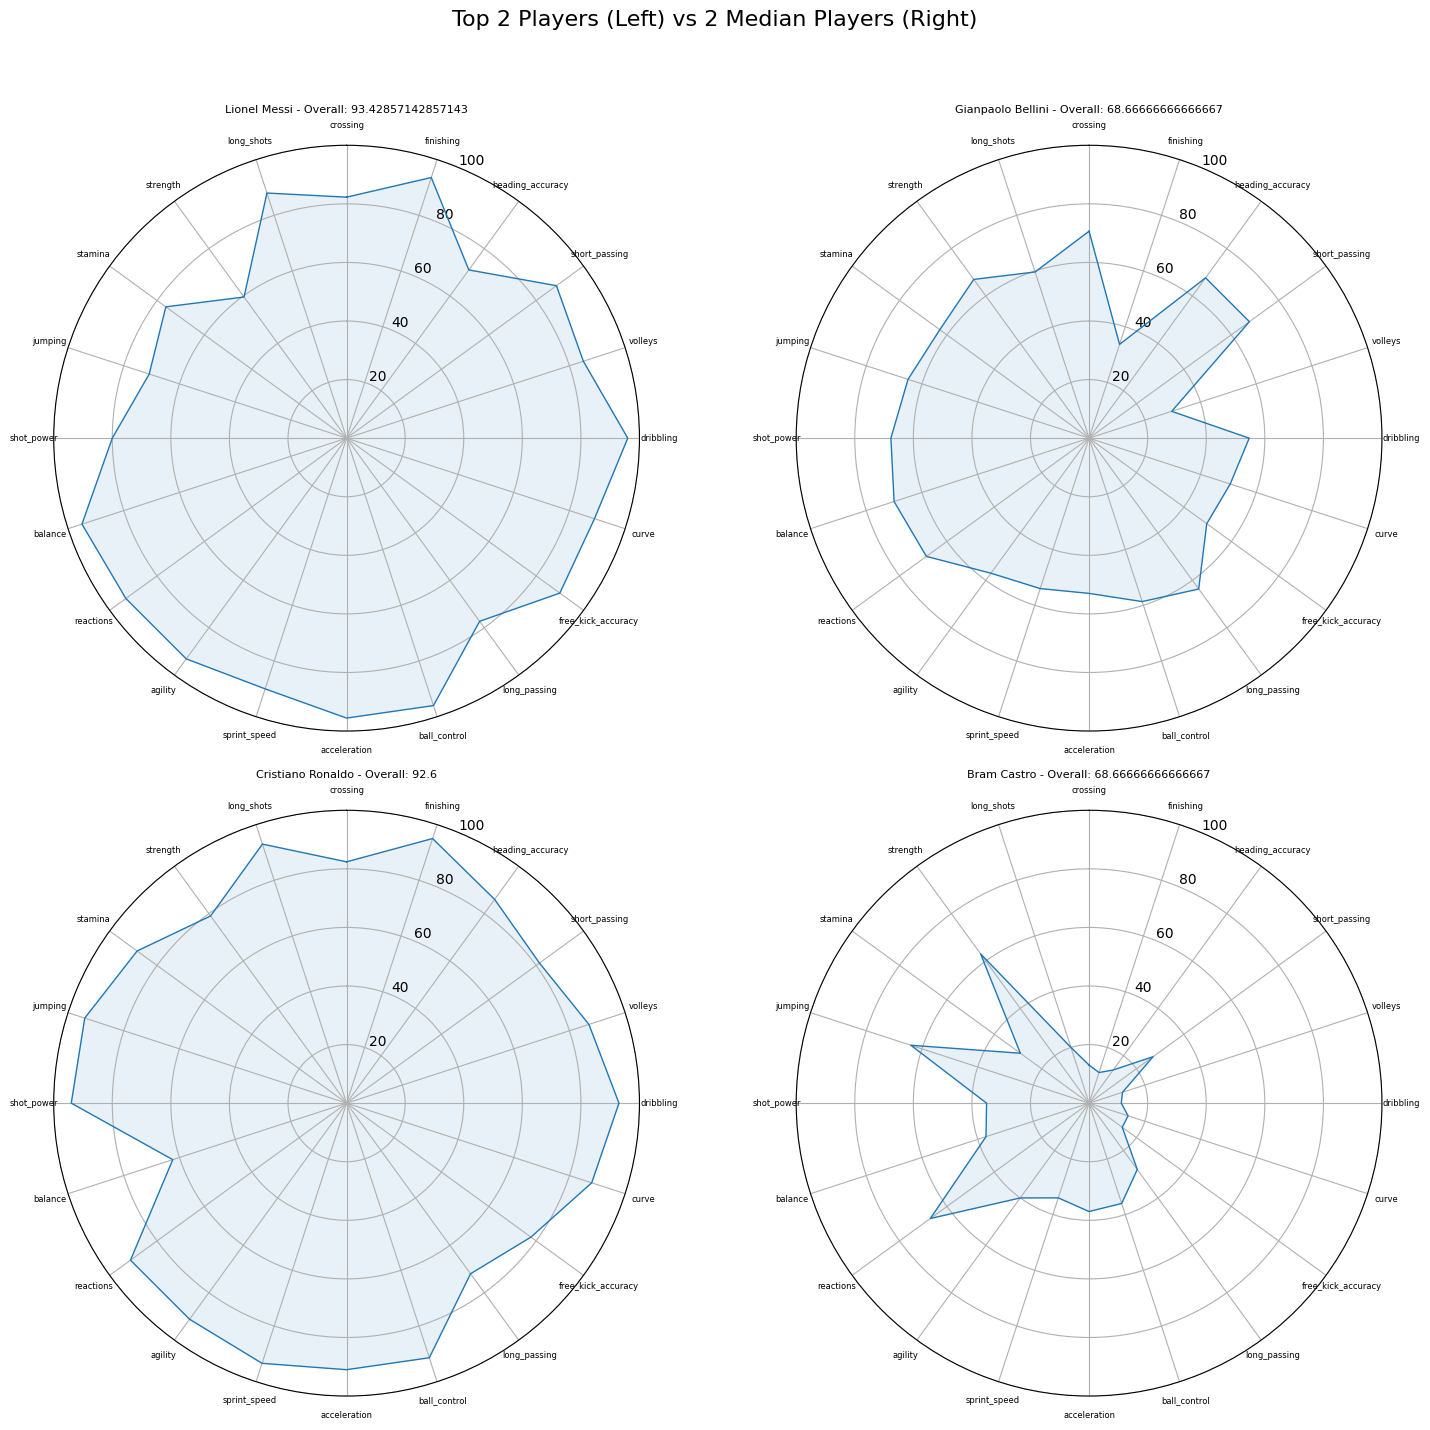
\includegraphics[width=0.6\linewidth]{radar_plot.png}
    \caption{Radar plot comparing top-rated players versus average players, here top players exhibit a more balanced skill profile across multiple attributes}
    \label{fig:radar_plot}
\end{figure}
\begin{figure}
    \centering
    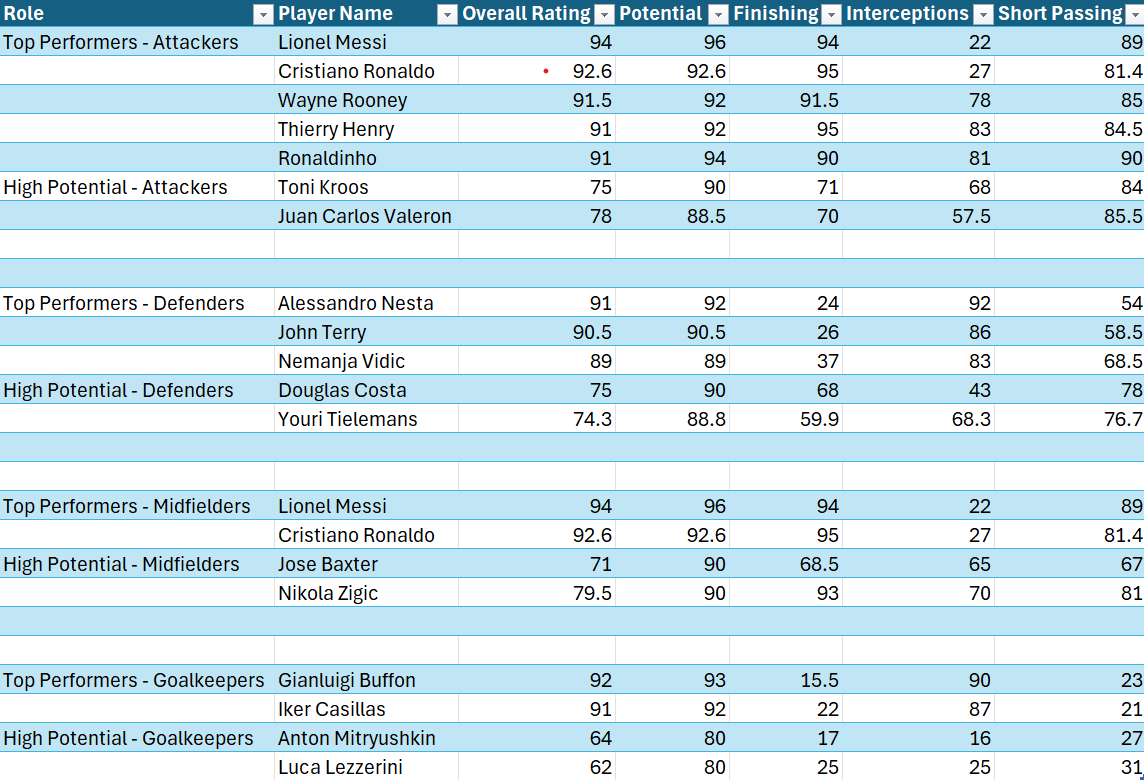
\includegraphics[width=1\linewidth]{key_players.png}
\caption{Player Transfer Recommendations by Role}
    \label{fig:player_recommendations}
\end{figure}
\subsection{Player Transfer Recommendations}

To address Hypothesis 2, we leveraged player and team performance data to identify weaknesses in the team and propose potential player transfers to optimize team performance. The results, as shown in Figure~\ref{fig:player_recommendations}, provide a list of high-performing players and high-potential players for each role. These predictions align with observed player strengths and league-specific needs.

Key findings for a team like Liverpool showed us that they were weak in attack, and the players were predicted like below:
\begin{itemize}
    \item \textbf{Attackers:} Lionel Messi and Cristiano Ronaldo are identified as top-performing attackers with balanced attributes like finishing and short passing. High-potential players like Toni Kroos and Juan Carlos Valeron are highlighted for their potential to grow into impactful roles.
    \item \textbf{Defenders:} Alessandro Nesta and John Terry lead as top defenders, excelling in interceptions and short passing. High-potential players like Douglas Costa and Youri Tielemans offer promising defensive skills to strengthen weak backlines.
\end{itemize}
While these recommendations are subjective, they align with realistic player profiles. Toni Kroos, who has been identified as a high-potential attacker, is a reasonable suggestion given his skill set and current trajectory, which played out similarly in real life, when he moved to Real Madrid in a massive transfer and became a pivotal player for the team. Established stars like Messi and Ronaldo are naturally identified as top performers, validating the method's ability to reflect reality.

These results serve as a preliminary filter for scouts and recruiters, who can further validate and refine the recommendations. The predictions are not validated against specific metrics but demonstrate logical and accurate alignment with expected player strengths and team needs.

The results provided subjective but logical recommendations for player transfers, addressing the hypothesis. High-performing players and players with potential were identified based on their attributes, aligning well with real-world observations. However, the method lacks validation against real-world outcomes, which leaves room for improvement in the robustness of the recommendations.

The results are limited by subjectivity in roles because player roles are inferred based on a combination of attributes, which may not fully capture the nuances of real-world performance and also the recommendations did not consider tactical systems or financial constraints, which are critical in making actionable transfer decisions.

To refine the approach, we can develop metrics to quantify the impact of each attribute on specific roles. For instance, determine how “short passing” contributes to midfielders versus attackers, enabling more precise role classification. Next, we can also incorporate tactical styles into the recommendation process. For example, a team focusing on fast counterattacks may prioritize players with high pace and short-passing accuracy.We can also introduce financial metrics like transfer market value and salary demands into the analysis to align recommendations with real-world constraints.Finally we can, simulate team performance with the recommended transfers to evaluate their impact before making final suggestions.

%%%%%%%%%%%%%%%%%%%%%%%%%%%%%%%%%%%%%%%%%%%%%%%%%%%%%%%%%%%%%%%%%
%%%%%%%%%%%%%%%%%%%%% --- SECTION START --- %%%%%%%%%%%%%%%%%%%%%
%%%%%%%%%%%%%%%%%%%%%%%%%%%%%%%%%%%%%%%%%%%%%%%%%%%%%%%%%%%%%%%%%
\section{Conclusions}

\subsection{Lessons Learned}

This project provided valuable insights into both the problem domain of soccer analytics and the methodologies employed to address predictive tasks. Key lessons learned are give below:

\begin{itemize}
    \item \textbf{Complexity of Match Outcome Prediction:} Predicting match outcomes, particularly for the "Draw" class, highlighted the inherent challenges of imbalanced datasets. This reinforced the importance of addressing class imbalance through methods such as cost-sensitive learning, oversampling, or synthetic data generation. Additionally, it became evident that match outcomes are influenced by many dynamic factors beyond the features available in the dataset, such as psychological and tactical elements.

    \item \textbf{Nuances of Player Evaluation:} Player performance metrics, while useful, provided only a partial view of a player's role and potential. The subjective nature of evaluating attributes like "potential" underscored the importance of combining quantitative analysis with expert domain knowledge. This project emphasized that while data-driven insights are powerful, they must be contextualized within the broader scouting process.

    \item \textbf{Importance of Feature Engineering:} The EDA and feature engineering process showed us the critical role of deriving meaningful features, such as team ratings and tactical attributes. These features were instrumental in guiding the models, particularly for player transfer recommendations. This experience demonstrated that effective feature design often has as much impact as the choice of modeling techniques.

    \item \textbf{Limitations of Predictive Models in Decision-Making:} While models like Random Forest and Neural Networks can provide actionable predictions, their limitations in handling subjective decisions, such as player transfers, were apparent. The project reinforced the need for integrating prescriptive modeling approaches, such as optimization-based strategies or simulation, to complement predictive analytics.

\end{itemize}

\subsection{Unexplored Ideas and Future Directions}

We checked on using metrics to evaluate the recommendations from players transfers, but it is hard to obtain real world data that can help us identify if our predictions were right or not, due to the inherent subjective nature of the recommendations. Looking ahead, several promising directions could enhance this work. Incorporating dynamic features, such as player form or injury history, could improve predictive accuracy through time-series or recurrent neural network models. Integrating financial constraints, such as transfer fees and budgets, would make transfer recommendations more practical. Establishing feedback loops with domain experts, simulating tactical adjustments, and exploring advanced methods like graph-based models or reinforcement learning could further enrich the insights and applicability of soccer analytics.


This project demonstrated the potential of data-driven approaches in soccer analytics while highlighting their limitations in capturing the full complexity of the sport. The key takeaway is that analytics must serve as a complementary tool, enhancing rather than replacing human judgment. Moving forward, the integration of richer datasets, advanced modeling techniques, and expert input will be critical to furthering the impact of analytics in soccer management.



%%%%%%%%%%%%%%%%%%%%%%%%%%%%%%%%%%%%%%%%%%%%%%%%%%%%%%%%%%%%%%%%%
%%%%%%%%%%%%%%%%%%%%% --- SECTION START --- %%%%%%%%%%%%%%%%%%%%%
%%%%%%%%%%%%%%%%%%%%%%%%%%%%%%%%%%%%%%%%%%%%%%%%%%%%%%%%%%%%%%%%%
\printbibliography
\\~\\
The code is available in the GitHub repository \underline{\textcolor{blue}{\href{https://github.ncsu.edu/arao23/engr-ALDA-Fall2024-P28}{here}}}. 
\normalsize

\end{document}


\begin{figure}
    \centering
    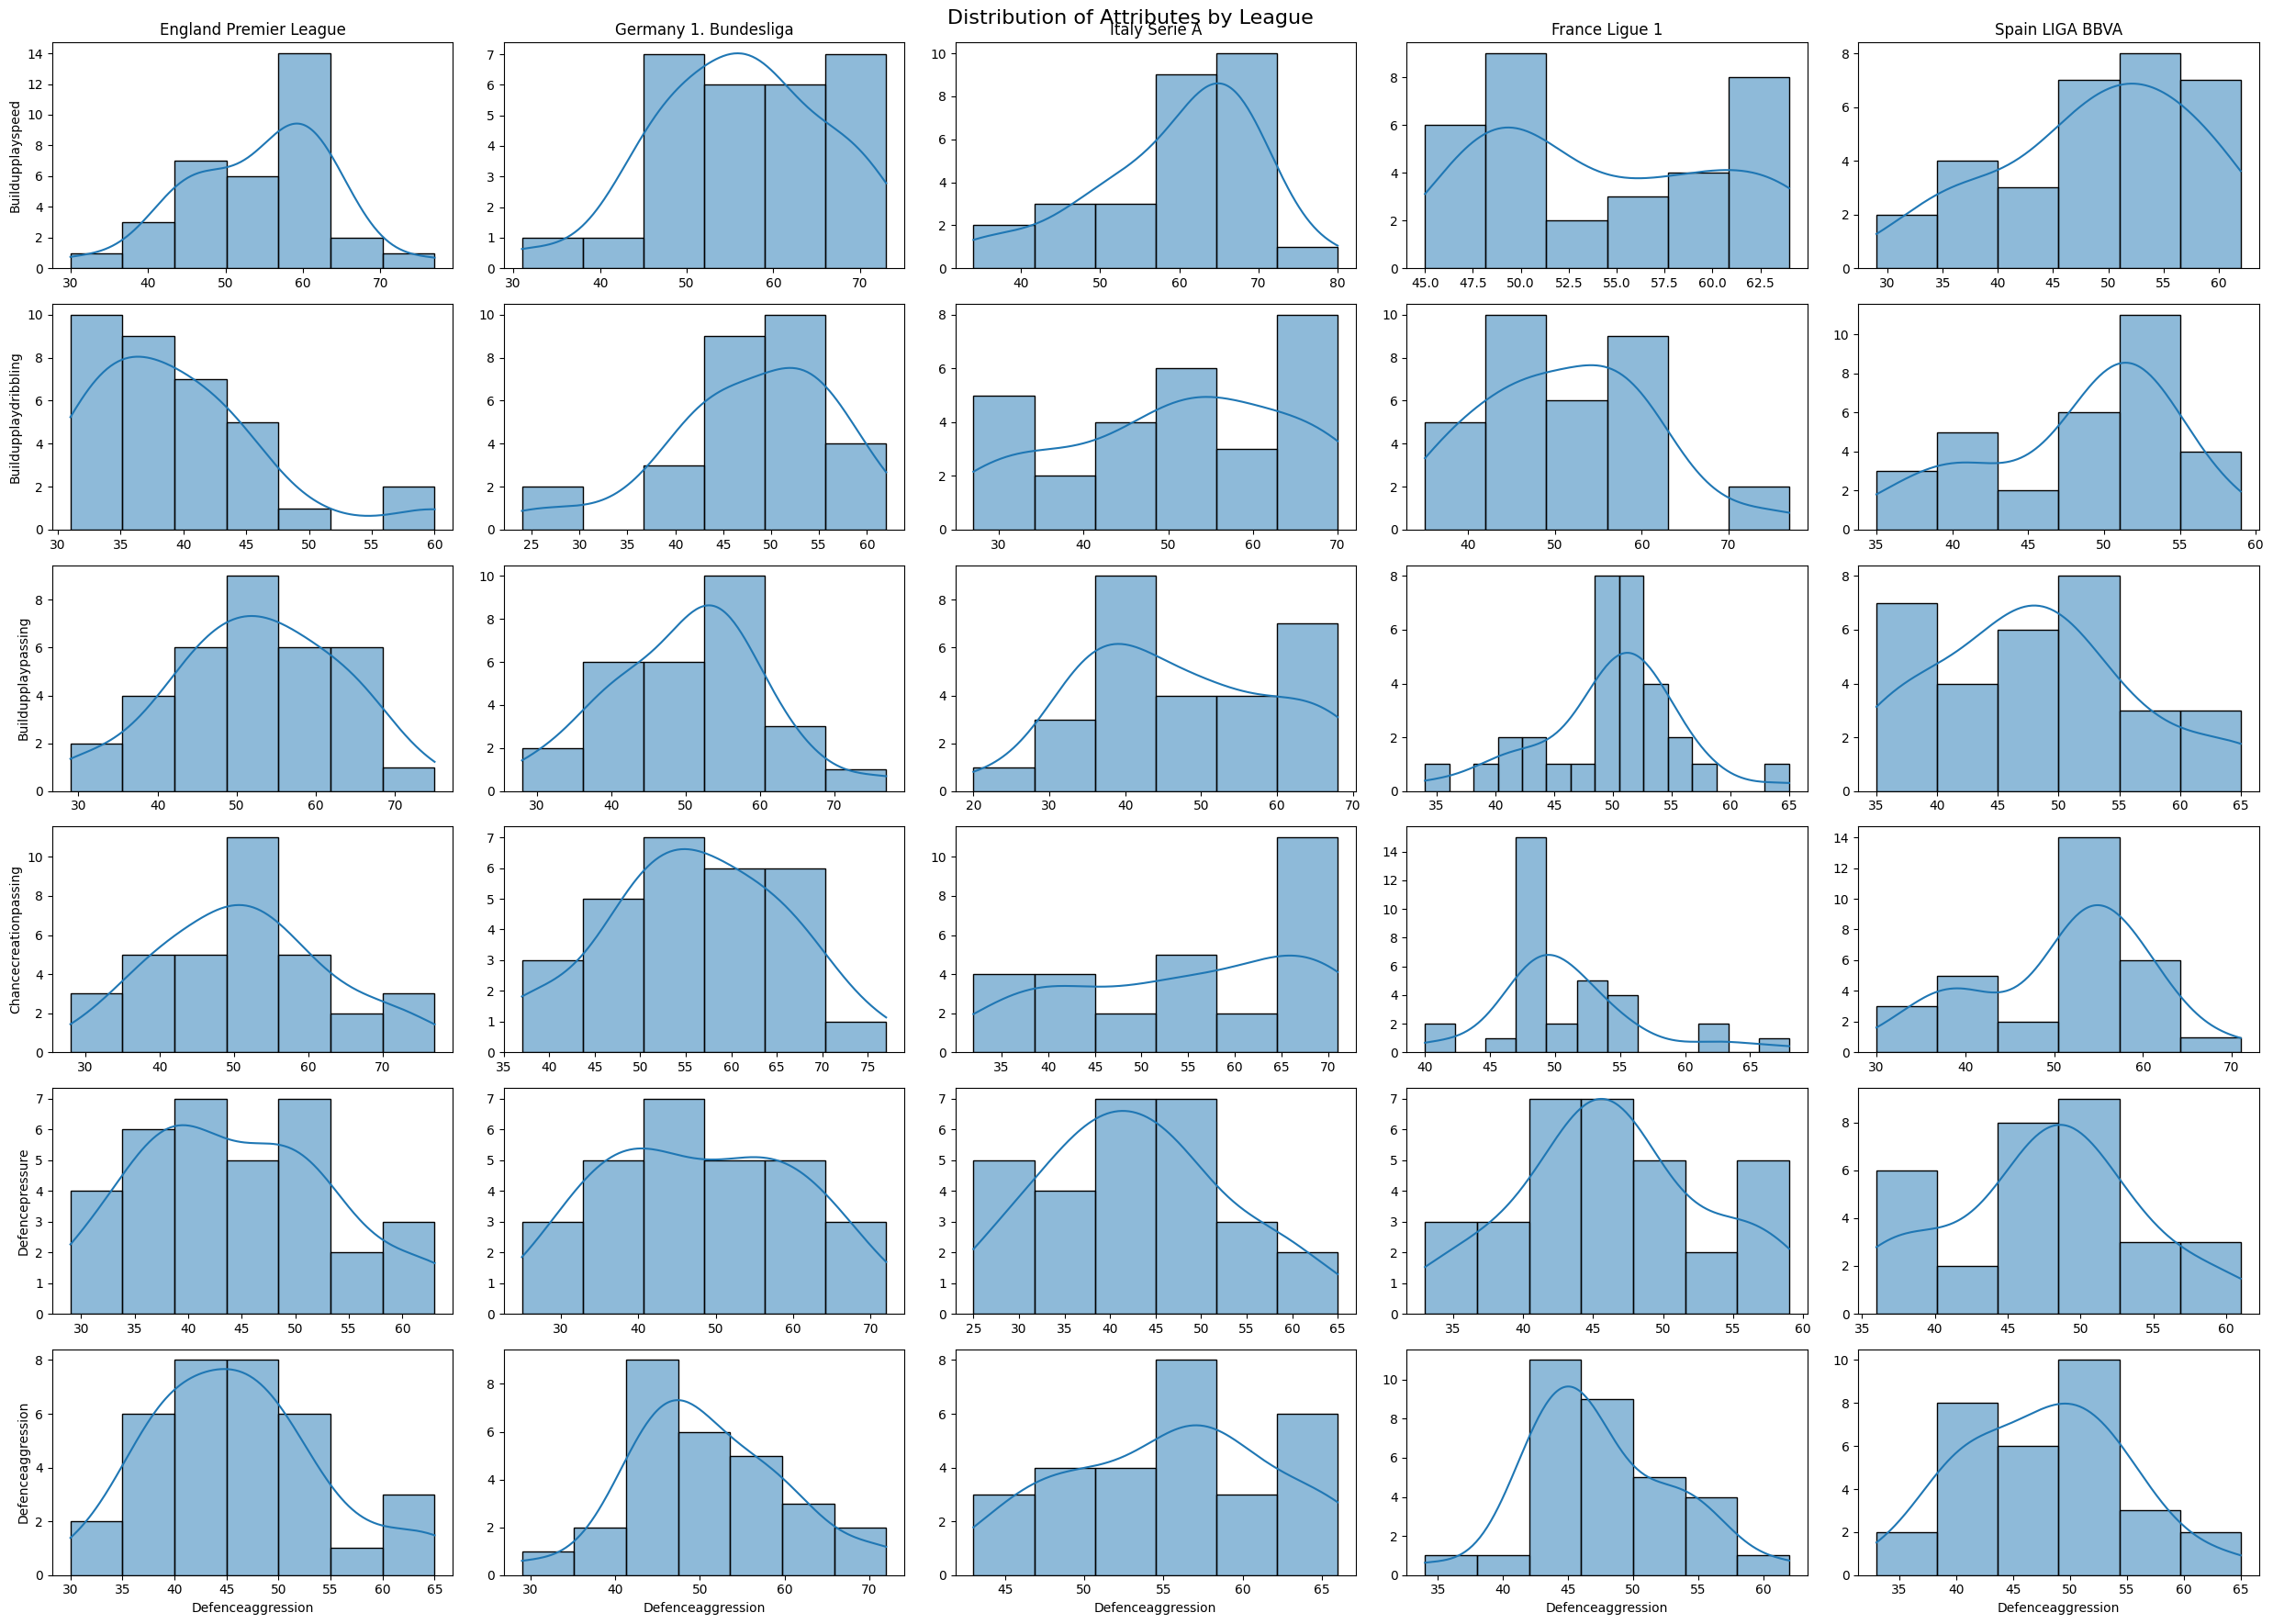
\includegraphics[width=0.7\linewidth]{league_features.png}
    \caption{League styles vary: La Liga focuses on passing, Bundesliga on speed, Ligue 1 on defense}
    \label{fig:enter-label}
\end{figure}